\begin{frame}{4.1 Inisialisasi Register dan Sirkuit Validasi}
    \begin{columns}
        \begin{column}{0.45\textwidth}
            \centering
            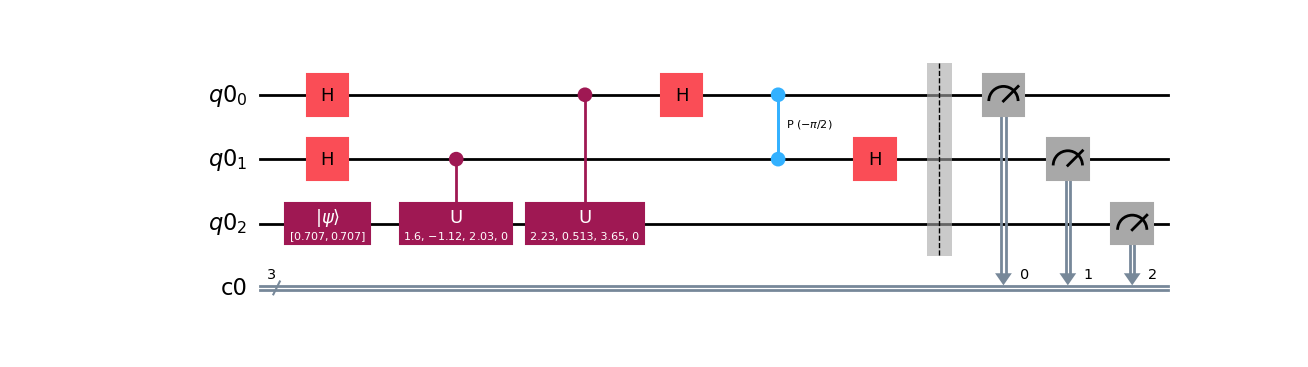
\includegraphics[width=\textwidth]{../QPCA-master/circuit_eigenstate.png}
            \captionof{figure}{Sirkuit Validasi 2-bit Phase}
        \end{column}
        \begin{column}{0.55\textwidth}
            \small
            \begin{itemize}
                \item \textbf{Target State:} Qubit target ($q_2$) disiapkan dalam \textit{eigenstate} murni $|+\rangle$.
                \item \textbf{Konfigurasi:} Menggunakan 2 qubit register fase ($q_0, q_1$) guna meminimalkan akumulasi galat gerbang.
                \item \textbf{Tujuan:} Memverifikasi ketajaman interferensi konstruktif pada sistem dengan kedalaman sirkuit rendah.
            \end{itemize}
        \end{column}
    \end{columns}
\end{frame}

\begin{frame}{4.2 Dekomposisi Sirkuit: Transpiled Eigenstate}
    \begin{columns}
        \begin{column}{0.6\textwidth}
            \centering
            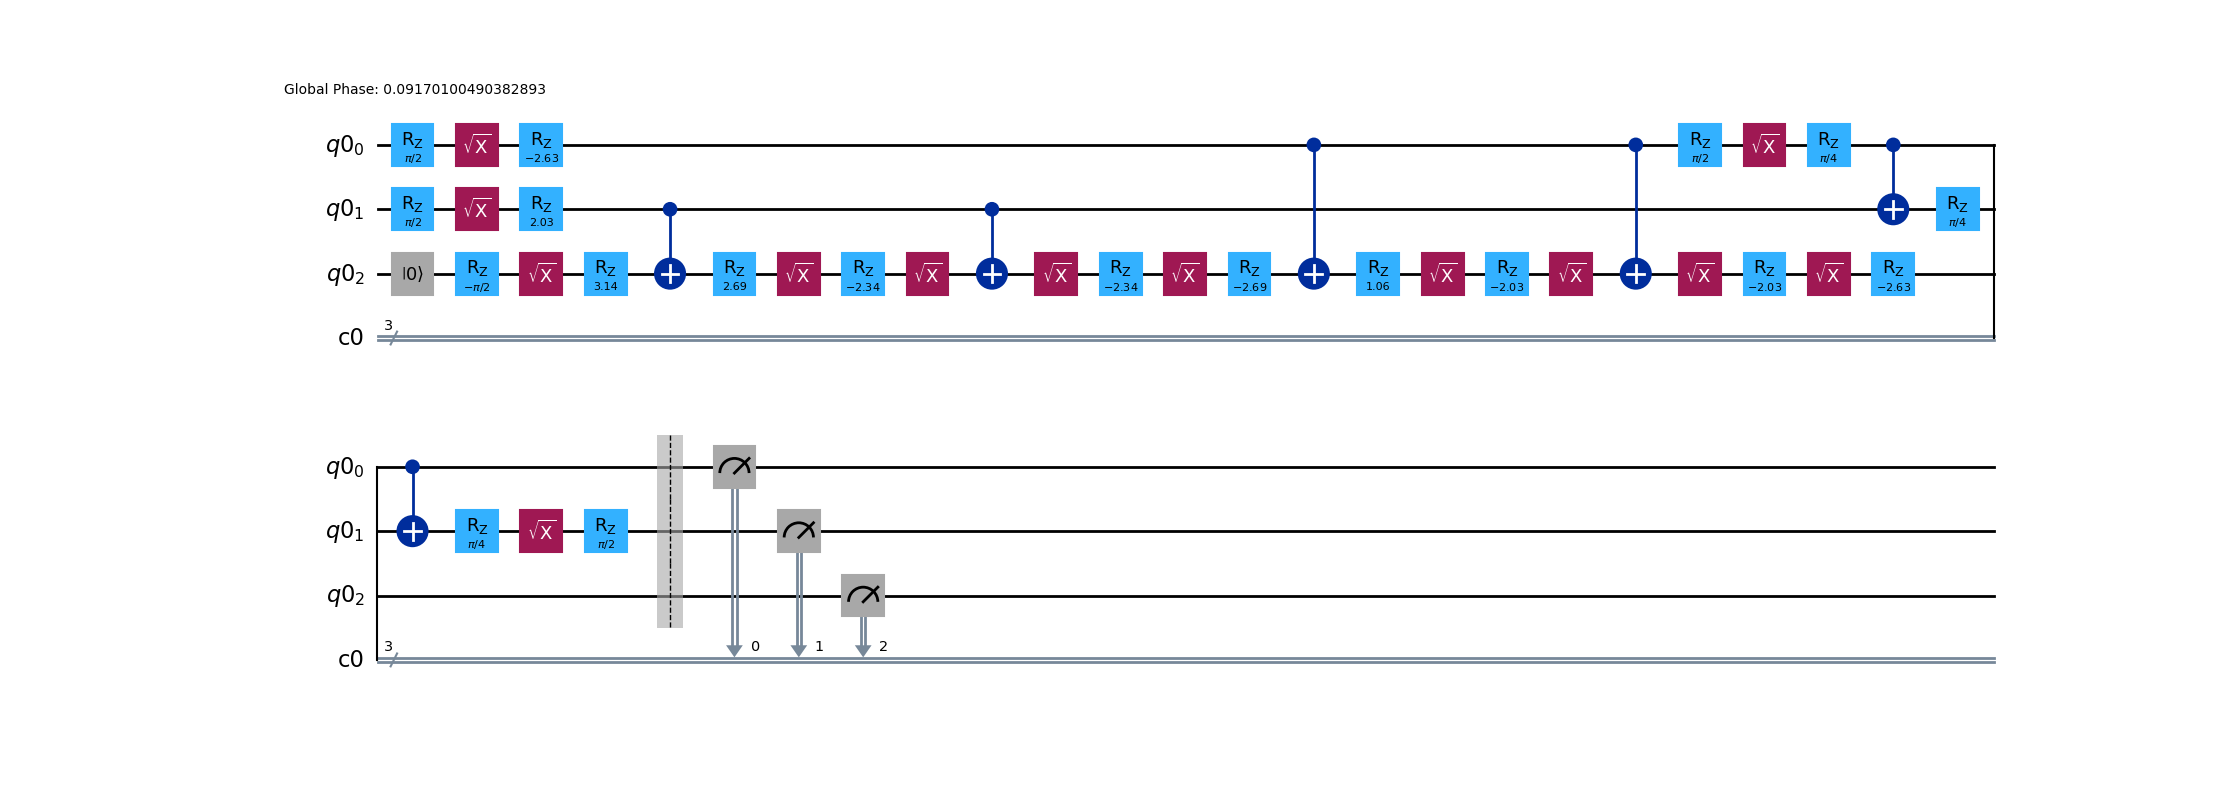
\includegraphics[width=\textwidth]{../QPCA-master/circuit_transpiled_eigenstate.png}
            \captionof{figure}{Sirkuit Validasi setelah Transpilasi}
        \end{column}
        \begin{column}{0.4\textwidth}
            \small
            \begin{itemize}
                \item \textbf{Optimasi Gerbang:} Transpilasi menyederhanakan rangkaian gerbang menjadi instruksi dasar yang kompatibel dengan arsitektur qubit spesifik.
                \item \textbf{Fidelitas Tinggi:} Kedalaman sirkuit yang relatif dangkal pada tahap ini menjamin integritas informasi fase tetap terjaga selama eksekusi.
                \item \textbf{Pemetaan Fisik:} Memberikan visualisasi bagaimana register target dan fase berinteraksi melalui gerbang CNOT pada level perangkat keras.
            \end{itemize}
        \end{column}
    \end{columns}
\end{frame}

\begin{frame}{4.3 Hasil Pengukuran: Konvergensi Fase 2-bit}
    \begin{columns}
        \begin{column}{0.5\textwidth}
            \centering
            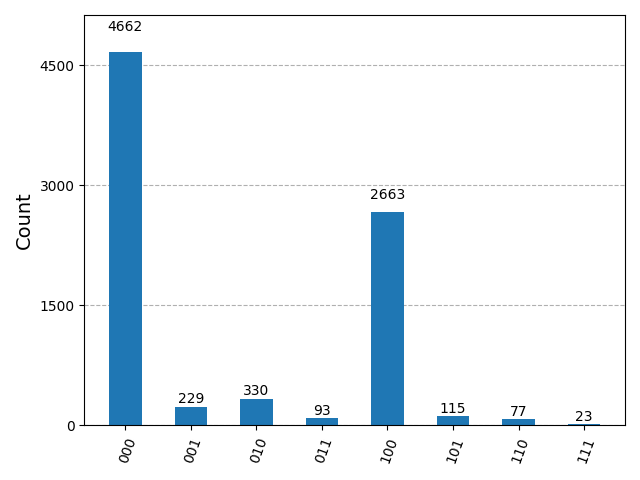
\includegraphics[width=\textwidth]{../QPCA-master/qpca_eigenstate_result.png}
            \captionof{figure}{Histogram Probabilitas Eigenstate}
        \end{column}
        \begin{column}{0.5\textwidth}
            \small
            \begin{itemize}
                \item \textbf{Ketajaman Puncak:} Histogram menunjukkan puncak yang sangat terfokus pada satu state biner.
                \item \textbf{Supresi Noise:} Probabilitas pada state non-target hampir nol, mengonfirmasi interferensi destruktif optimal.
                \item \textbf{Akurasi:} Memberikan tingkat kepercayaan tinggi terhadap parameter rotasi $(\theta, \phi, \lambda)$ yang digunakan.
            \end{itemize}
        \end{column}
    \end{columns}
\end{frame}

\begin{frame}{4.4 Analisis Matriks Densitas: State City Eigenstate}
    \begin{columns}
        \begin{column}{0.5\textwidth}
            \centering
            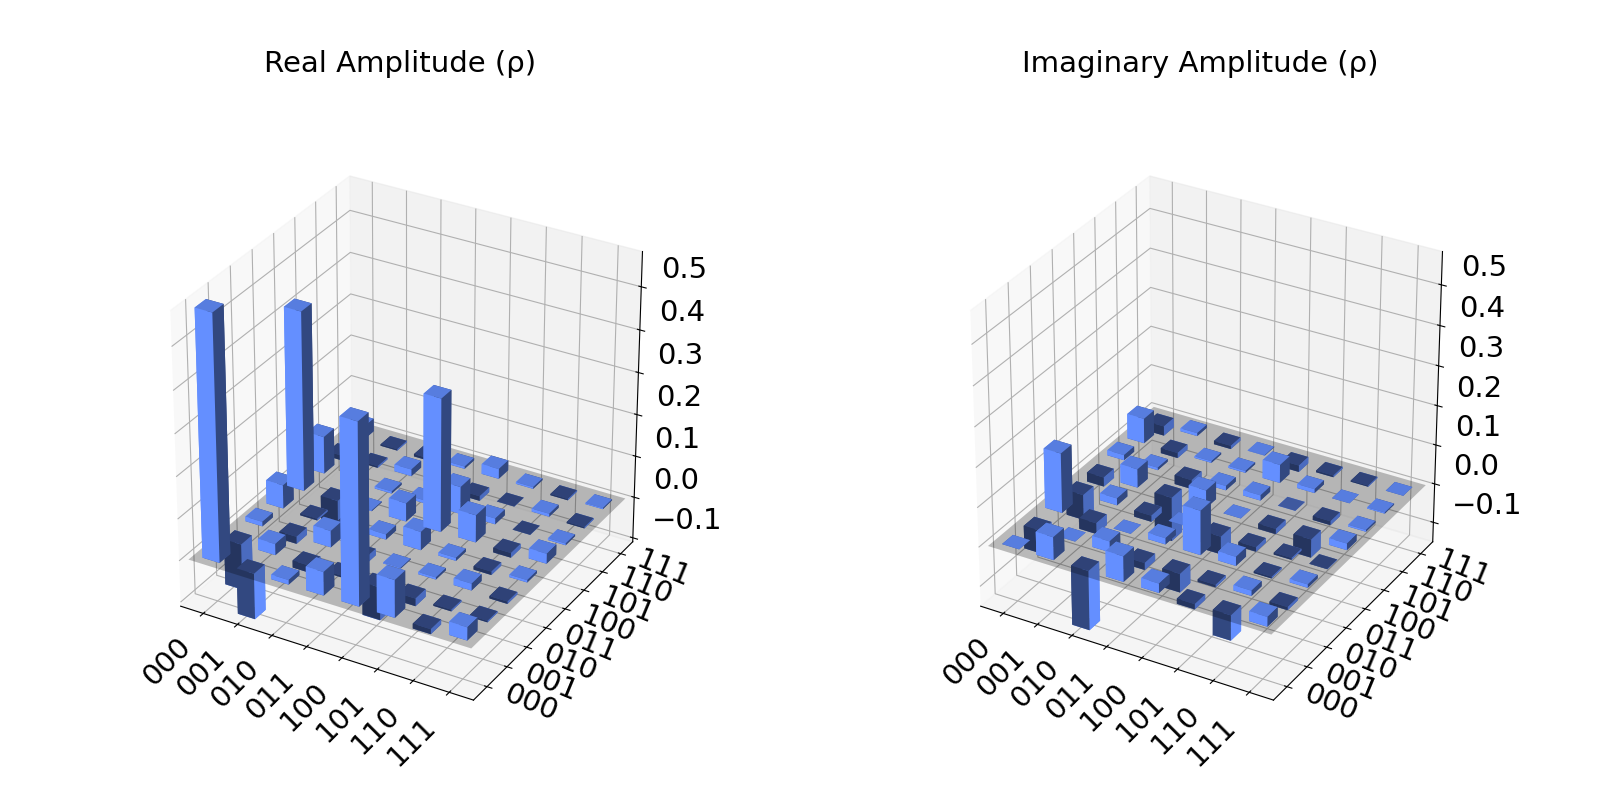
\includegraphics[width=\textwidth]{../QPCA-master/state_city_eigenstate.png}
            \captionof{figure}{State City Validasi (Elemen Riil)}
        \end{column}
        \begin{column}{0.5\textwidth}
            \small
            \begin{itemize}
                \item \textbf{Struktur Bar:} Menunjukkan bar utama pada diagonal yang menandakan kemurnian \textit{state} yang tinggi.
                \item \textbf{Integritas State:} Distribusi amplitudo yang terpusat mengonfirmasi stabilitas fase tanpa kebocoran informasi.
            \end{itemize}
        \end{column}
    \end{columns}
\end{frame}

\begin{frame}{4.5 Pemetaan Korelasi pada Hinton Map Eigenstate}
    \begin{columns}
        \begin{column}{0.5\textwidth}
            \centering
            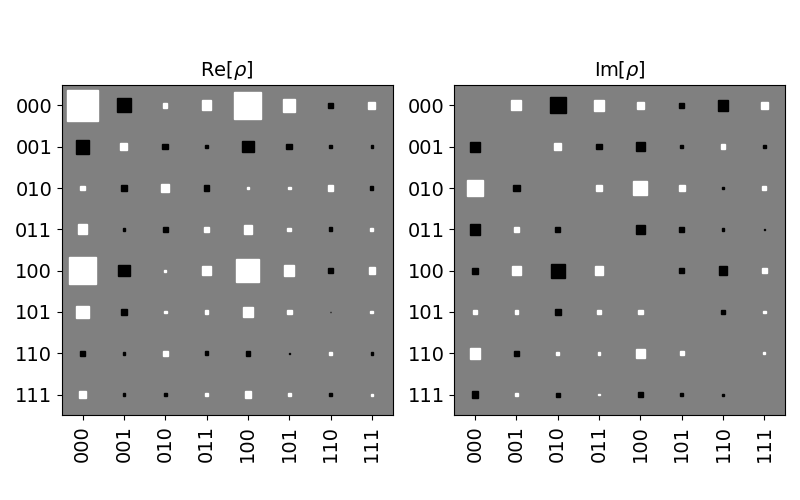
\includegraphics[width=0.9\textwidth]{../QPCA-master/hinton_eigenstate.png}
            \captionof{figure}{Hinton Map: Fokus Entanglement}
        \end{column}
        \begin{column}{0.5\textwidth}
            \small
            \begin{itemize}
                \item \textbf{Distribusi Kotak:} Ukuran kotak putih yang besar menunjukkan korelasi sangat kuat antara register fase dan input.
                \item \textbf{Kontras Visual:} Bukti empiris keberhasilan protokol \textit{phase kickback} dalam memetakan profil spektral dengan presisi tinggi.
            \end{itemize}
        \end{column}
    \end{columns}
\end{frame}

\begin{frame}{4.6 Verifikasi Geometris pada Bola Bloch Eigenstate}
    \begin{columns}
        \begin{column}{0.5\textwidth}
            \centering
            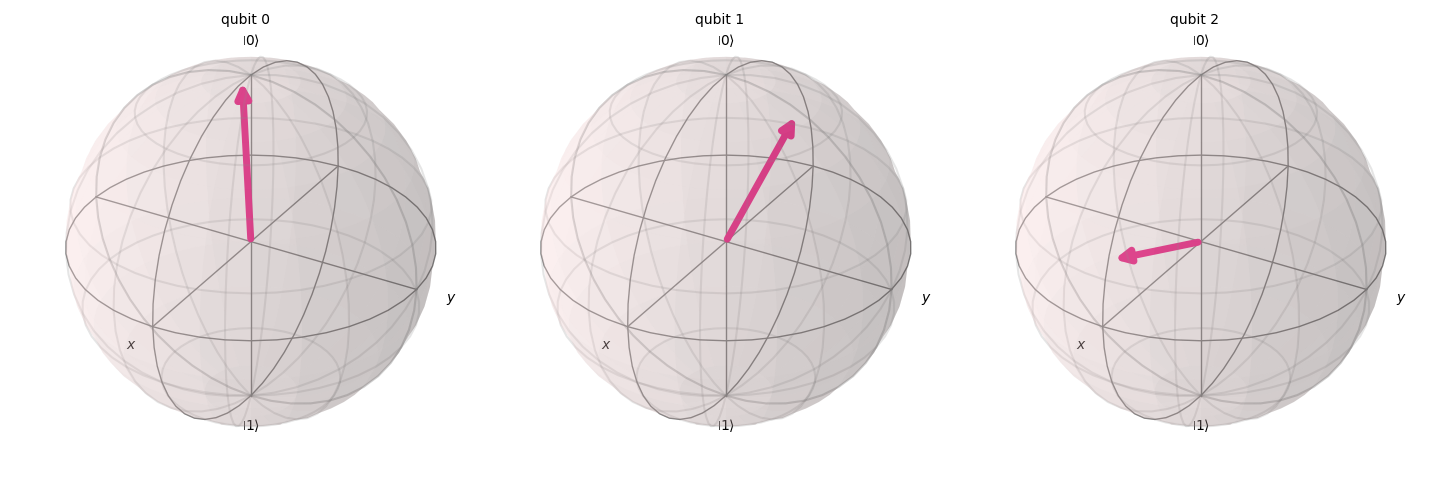
\includegraphics[width=\textwidth]{../QPCA-master/bloch_eigenstate.png}
            \captionof{figure}{Multivektor Bloch: Kondisi Ideal}
        \end{column}
        \begin{column}{0.5\textwidth}
            \small
            \begin{itemize}
                \item \textbf{Orientasi Statis:} Seluruh vektor mengarah presisi ke permukaan bola ($r \approx 1$).
                \item \textbf{Konsistensi Qubit:} Qubit target $q_2$ mempertahankan orientasi $|+\rangle$, memverifikasi integritas \textit{eigenstate} input.
                \item \textbf{Stabilitas:} Ketiadaan deviasi pada sumbu z menunjukkan sistem bebas dari galat fasa sistemik.
            \end{itemize}
        \end{column}
    \end{columns}
\end{frame}
